To produce a PCB, the layout design is transmitted to a manufacturer and a finished PCB is shipped.  The standard method of sharing layout design files between the designer and manufacturer is the text-based Gerber and Excellon drill file formats.  Still, there are enough variations in file naming, packaging, number format, and drill files that the manufacturer's requirements and EDA suite capabilities need to be carefully scrutinized.  Advanced Circuits is capable of receiving Gerber files in the newer 247X format, Excellon drill files, and Gerber FAB files~\cite{AdvCirFile, AdvCirGerMis, AdvCirFreeDFMCheck}.  The company also offers an automated Gerber file review and quoting service that can increase confidence in the successful manufacturing of the PCB design~\cite{AdvCirFreeDFMCheck}.  The procedure for creating the design files required for the Advanced Circuits manufacturing services is elucidated in Appendix~\ref{sec:gerberexp}.

A PCB is useless without components with which to populate the board.  Table~\ref{tab:bom} in Appendix~\ref{sec:bom} shows the bill of materials required to populate the Electrophysiology Interface board.  Components may be ordered from electronics supplier DigiKey\textsuperscript{\textregistered}, and the table includes the supplier part numbers and prices as of March 2013.  Components for the Electrophysiology Interface board are sourced from DigiKey\textsuperscript{\textregistered} along with samples provided by Analog Devices\textsuperscript{\textregistered} and Linear Technology\textsuperscript{\textregistered}.

After the PCB and components are received, assembly is required.  Components are populated by soldering them to the board by hand.  Logical circuit blocks, as defined in the subsections of section~\ref{sec:hardware}, are populated together while constantly testing for unintended short and open circuit conditions by using a resistance meter and by powering the board after each logical block is populated.  Soldering the most difficult components of the logical block first, such as ICs, is a good strategy to allow the best possible access to the hard to see and reach pins.  Pictures of the assembled Electrophysiology Interface board can be seen in Figures~\ref{fig:eitop} and~\ref{fig:eibot}.

\begin{figure}[H]
	\begin{singlespace}
	\centering	
		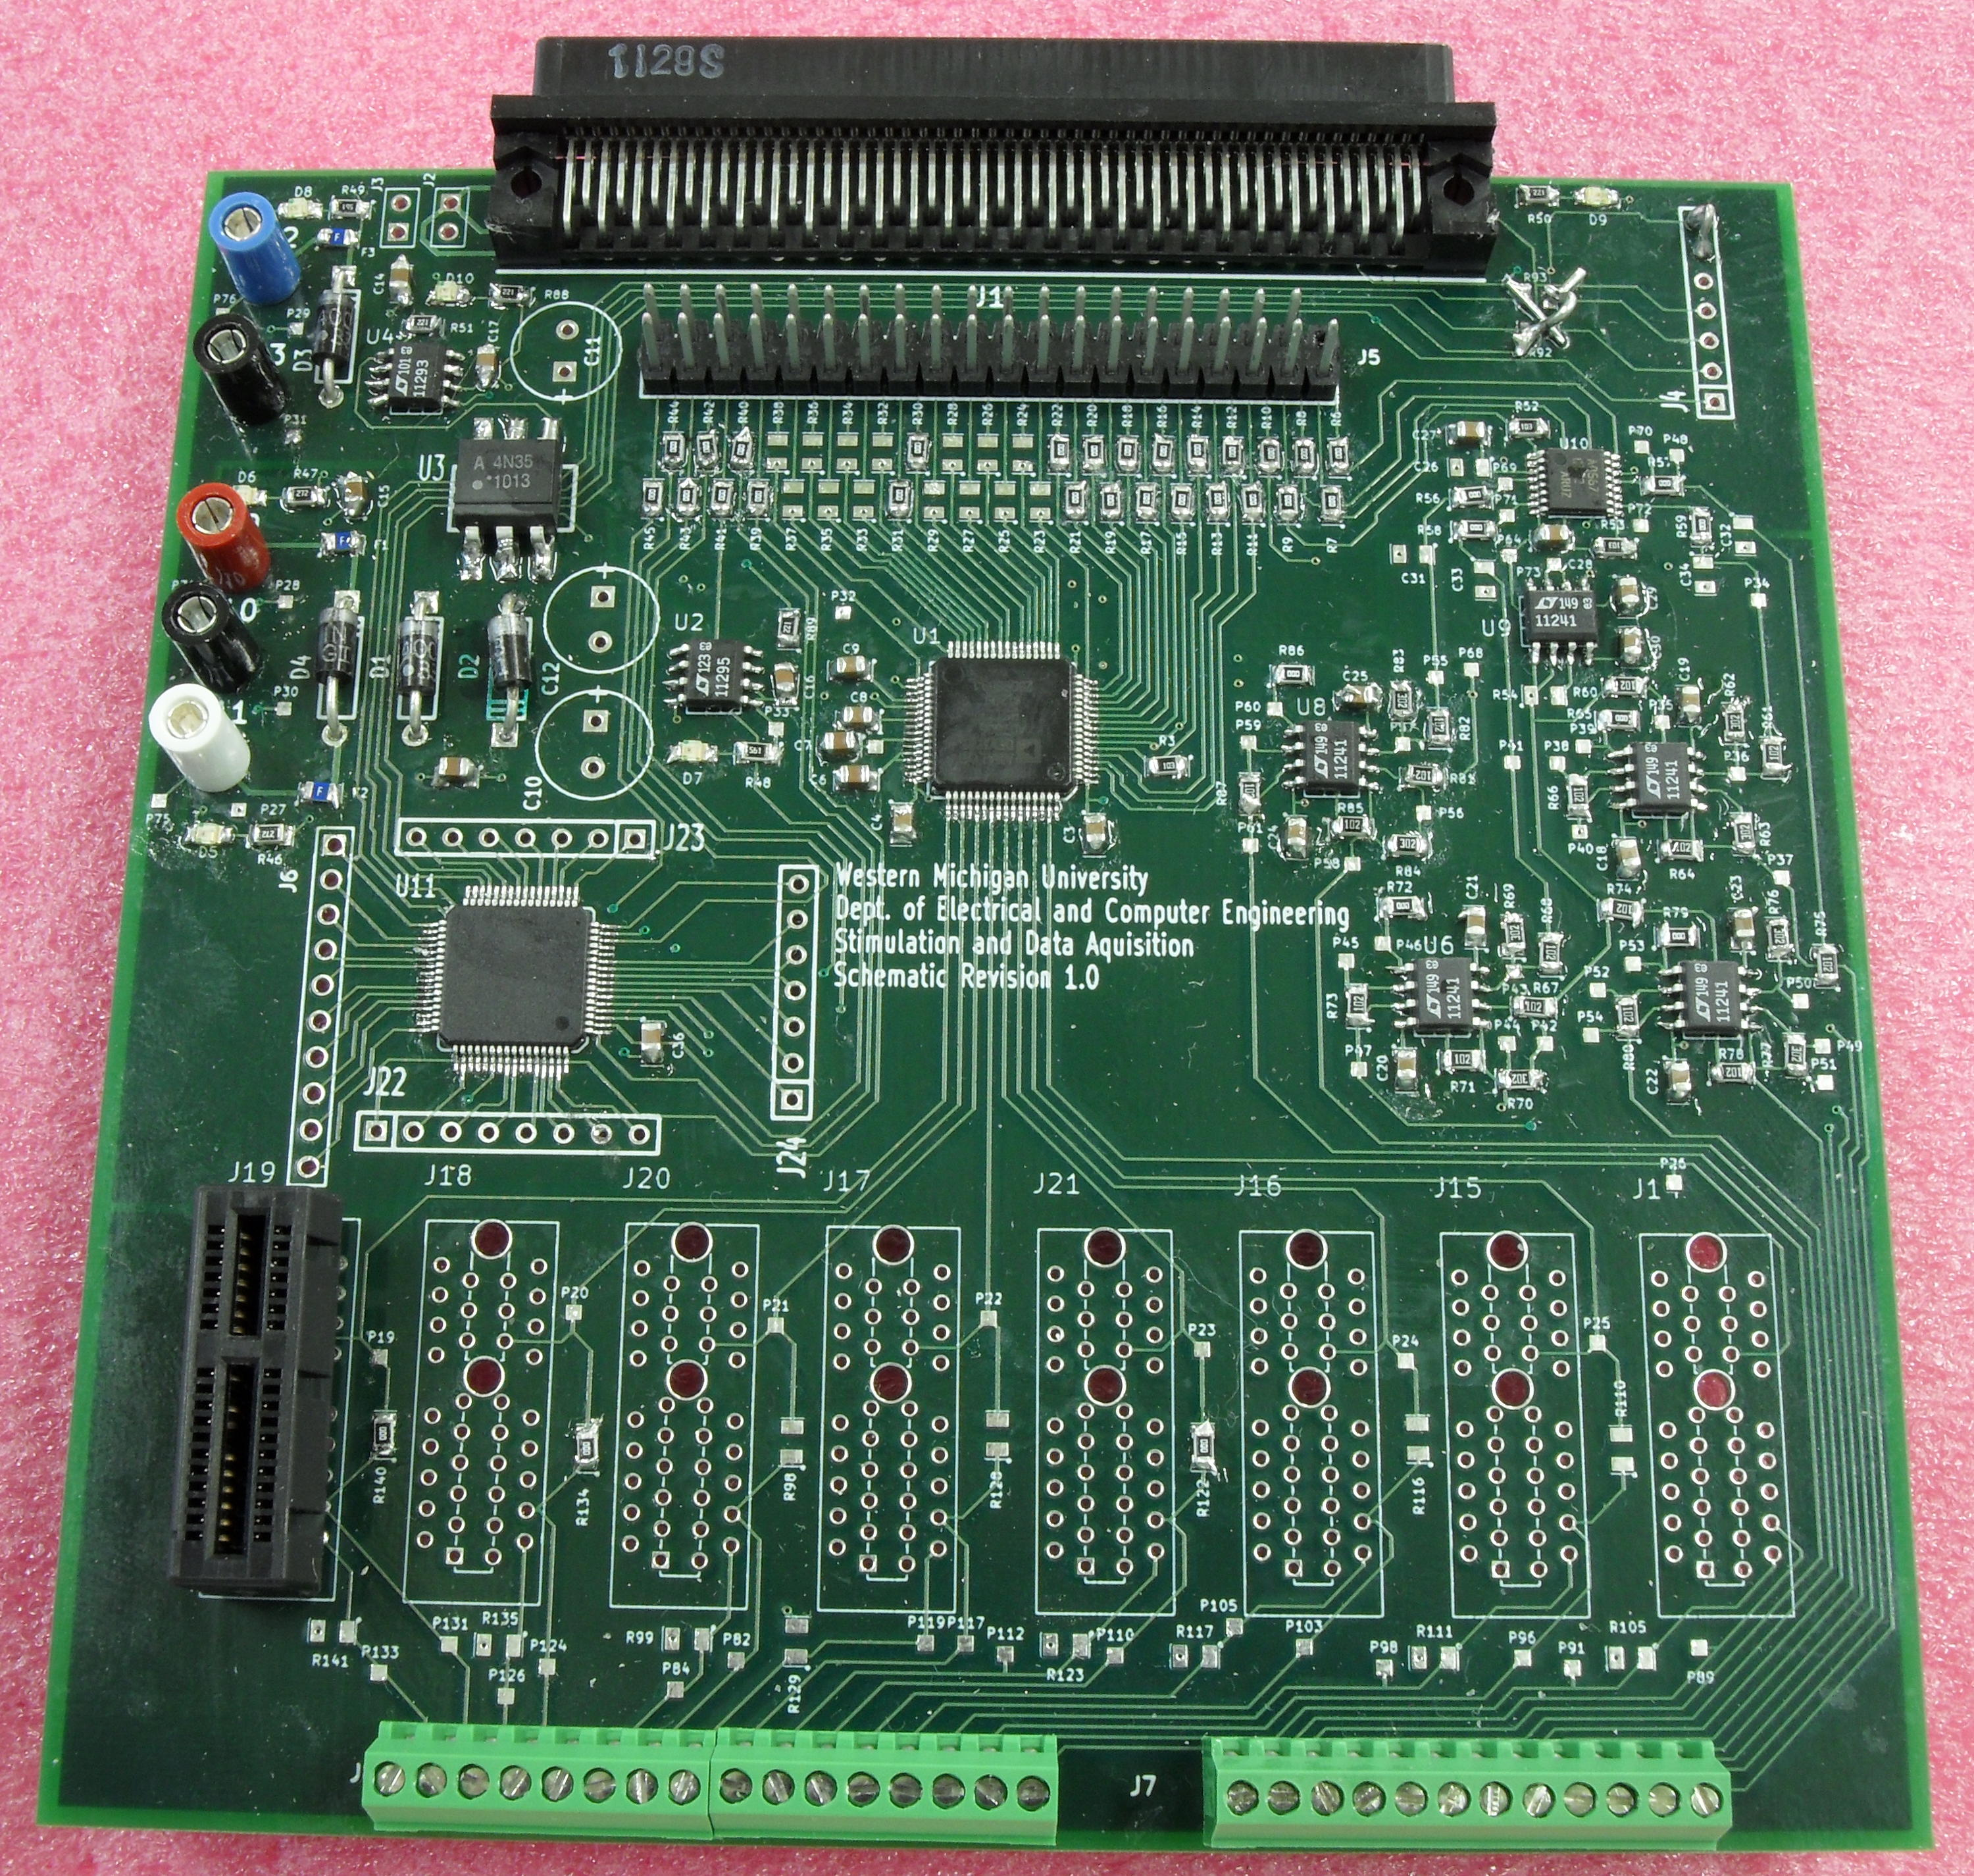
\includegraphics{./figures/EITop} 
	\caption{View of the top side of the populated Electrophysiology Interface board\label{fig:eitop}}
	\end{singlespace}
\end{figure}

\begin{figure}[H]
	\begin{singlespace}
	\centering	
		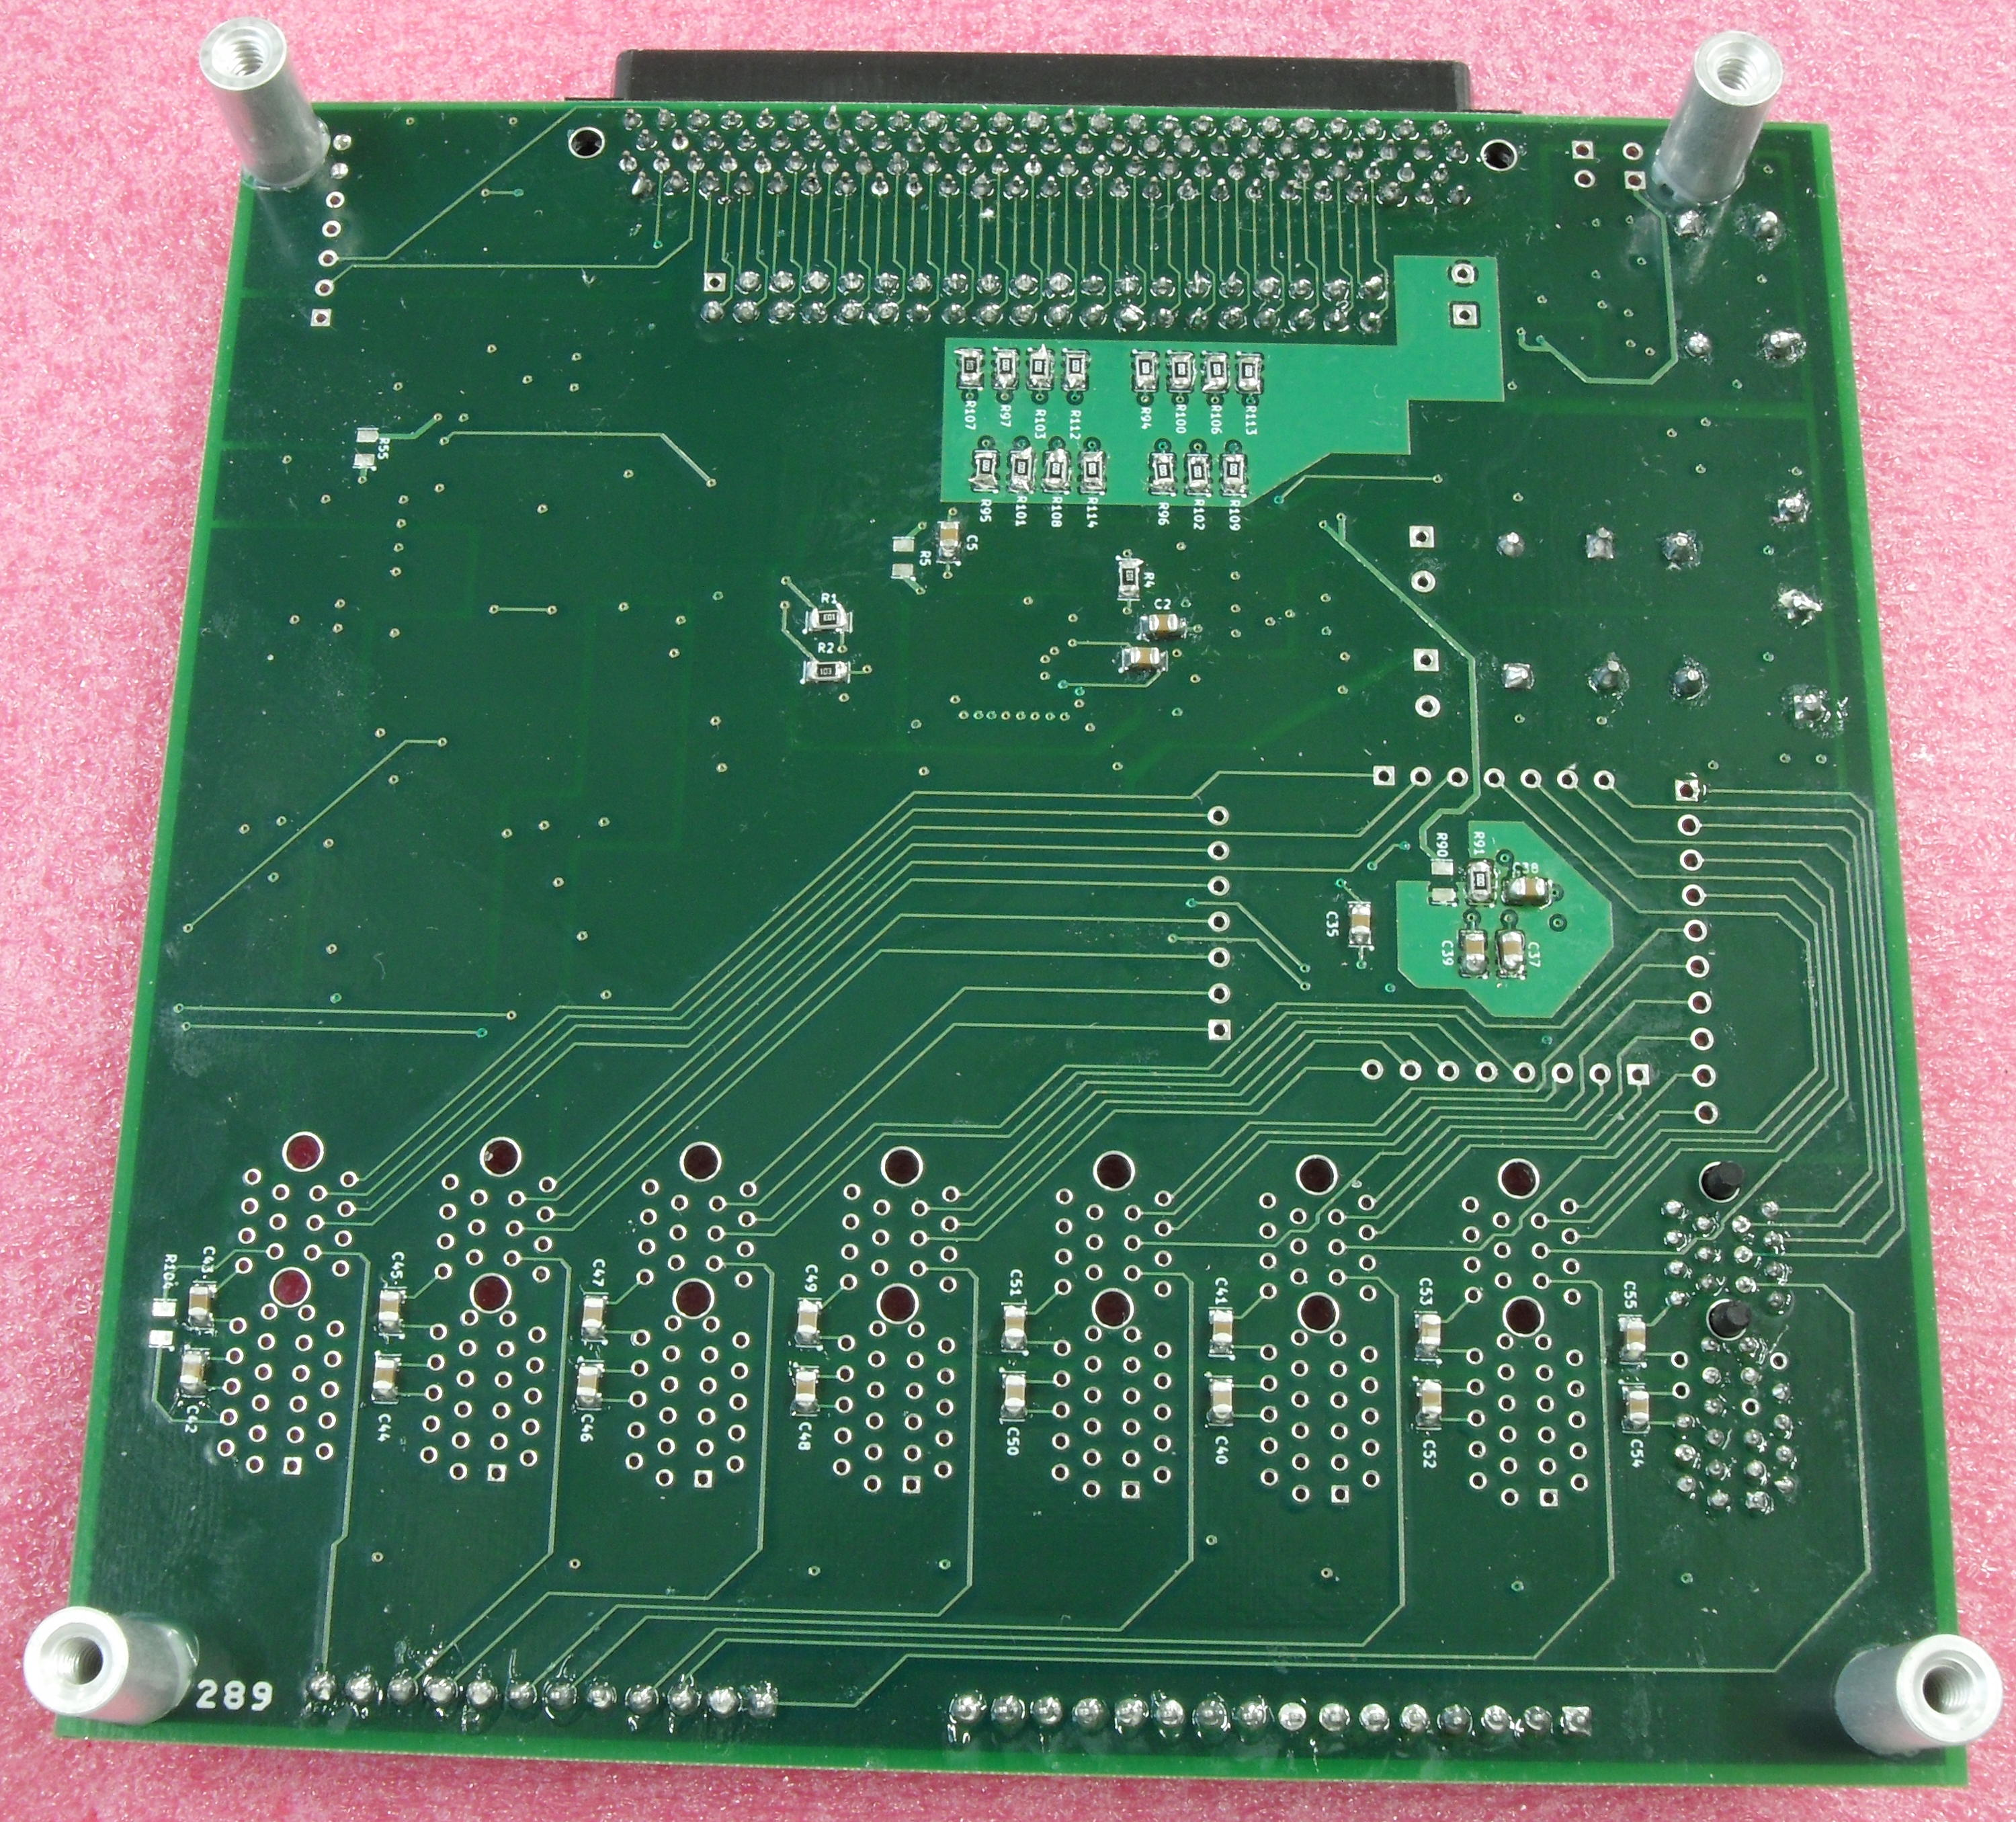
\includegraphics{./figures/EIBot} 
	\caption{View of the bottom side of the populated Electrophysiology Interface board\label{fig:eibot}}
	\end{singlespace}
\end{figure}
